\documentclass[
	article,
	11pt,
	oneside,
	a4paper,
	english,
	brazil,
	sumario=tradicional
	]{abntex2}

\usepackage{lmodern}
\usepackage[T1]{fontenc}
\usepackage[utf8]{inputenc}
\usepackage{indentfirst}
\usepackage{nomencl}
\usepackage{color}
\usepackage{graphicx}
\usepackage{microtype}
\usepackage[brazilian,hyperpageref]{backref}
\usepackage[alf]{abntex2cite}
\usepackage[makeroom]{cancel}
\usepackage{amsmath}
\graphicspath{{img/}}

\newcommand{\norm}[1]{\left\lVert#1\right\rVert}
\renewcommand{\backrefpagesname}{Citado na(s) página(s):~}
\renewcommand{\backref}{}
\renewcommand*{\backrefalt}[4]{
	\ifcase #1
		Nenhuma citação no texto.
	\or
		Citado na página #2.
	\else
		Citado #1 vezes nas páginas #2.
	\fi}

\titulo{Projeto 01 - Dinâmica na Ionosfera}
\tituloestrangeiro{}

\autor{Equipe Donner
\\[0.5cm]
Diogo Silva, Guilherme Shimada, Leonardo Vieira, Lucca Miranda, Pedro Azevedo}

\local{Brasil}
\data{30 de Agosto, 2021}

% alterando o aspecto da cor azul
\definecolor{blue}{RGB}{41,5,195}

\makeatletter
\hypersetup{
	pdftitle={\@title},
	pdfauthor={\@author},
	pdfsubject={Modelo de artigo científico com abnTeX2},
	pdfcreator={LaTeX with abnTeX2},
	pdfkeywords={abnt}{latex}{abntex}{abntex2}{atigo científico},
	colorlinks=true,
	linkcolor=blue,
	citecolor=blue,
	filecolor=magenta,
	urlcolor=blue,
	bookmarksdepth=4
}

\makeatother
\makeindex
\setlrmarginsandblock{3cm}{3cm}{*}
\setulmarginsandblock{3cm}{3cm}{*}
\checkandfixthelayout

\setlength{\parindent}{1.3cm}
\setlength{\parskip}{0.2cm}
\SingleSpacing

\begin{document}

\selectlanguage{brazil}
\frenchspacing

\twocolumn[ % INICIO DE ARTIGO EM DUAS COLUNAS
\maketitle

\begin{resumoumacoluna}
Este artigo apresenta uma discussão teórica a respeito do comportamento de partículas subatômicas carregadas da ionosfera. Para esse propósito, apresentaremos equações que modelam o ambiente em questão, a fim de melhor compreender a dinâmica dessas partículas quando as mesmas saem de uma situação de equilíbrio.

 \vspace{\onelineskip}

 \noindent
 \textbf{Palavras-chave}: ionosfera, força elétrica, oscilações, equações diferenciais.
\end{resumoumacoluna}
] % FIM DE ARTIGO EM DUAS COLUNAS

\textual
\section{Introdução}

O presente artigo propõe uma discussão teórica que tem como base uma situação problema que ocorre no plasma, conhecido como quarto estado físico da matéria. Ele é formado quando uma substância no estado gasoso é aquecida até atingir um valor tão elevado de temperatura que faz com que a agitação térmica molecular supere a energia de ligação que mantém os elétrons em órbita do núcleo atômico. Tal situação acontece nas camadas superiores da atmosfera terrestre, mais especificamente na ionosfera,e envolvendo o comportamento de partículas no interior dos metais.

Considerando um sistema neutro formado por elétrons livres e íons positivos (cátions), estando esses últimos fixos em sua posição; seguindo as leis de Newton; uma densidade volumétrica n0 igual para as duas cargas, queremos discutir física e matematicamente as consequências de um deslocamento do equilíbrio de cargas ao longo do eixo x. Além disso, precisamos discutir os efeitos que possam causar resistência ao movimento dos elétrons livres.

Inicialmente, a pesquisa está focada em encontrar uma equação que descreva a movimentação dos elétrons em torno dos íons positivos, mais especificamente a força restauradora que ´´atrai'' os elétrons para seu estado de equilíbrio. Ademais,os estudo também estão voltados para o encontro de um modelo simples que possa demonstrar efeitos resistivos dessa situação.

\section{Metodologia}

\subsection{Densidade final de carga}
Sabemos pelo enunciado que a densidade volumétrica de elétrons inicialmente é $n_0$. Tomando $N$ pelo número de elétrons naquela região, podemos expressar tal densidade da seguinte maneira:

\begin{equation} \label{densidade-eletronica-inicial}
  n_0 = \frac{N}{\Delta x}
\end{equation}

Assim, quando ocorre o deslocamente de densidade para fora do equilíbrio, temos a seguinte equação para a densidade eletrônica final:

\begin{equation} \label{densidade-eletronica-final}
  n_f = \frac{N}{\Delta x + \Delta s}
\end{equation}

Isolando a variável $N$ na equação~\ref{densidade-eletronica-inicial} e substituindo-a na equação~\ref{densidade-eletronica-final}, obtemos uma expressão de densidade eletrônica final que independe do número de elétrons:

\begin{equation}
  n_f = \frac{n_0\Delta x}{\Delta x + \Delta s}
\end{equation}

Note que podemos dividir o numerador e o denominador dessa fração por $\Delta x$, assim obtendo:

\begin{equation}
  n_f = \frac{n_0}{1 + \frac{\Delta s}{\Delta x}}
\end{equation}

Como $\frac{\Delta s}{\Delta x} \ll 1$, podemos usar a expansão de Taylor para aproximar a equação acima para outra mais conveniente:

\begin{equation} \label{densidade-eletronica-taylor}
  n_f = \frac{n_0}{1 + \frac{\Delta s}{\Delta x}} \approx n_0(1 - \frac{\Delta s}{\Delta x})
\end{equation}

A partir dessa equação de densidade de elétrons (de dimensão $\frac{\textrm{elétrons}}{m^3}$), podemos obter mudança de densidade de carga $\Delta\rho$ (de dimensão $\frac{\textrm{C}}{m^3}$) multiplicando a primeira por um fator dimensional $\frac{- q_e C}{\textrm{elétrons}}$, onde $q_e$ é a constante de carga elementar.

\begin{equation}
  \Delta\rho = \Delta n [\frac{\cancel{\textrm{elétrons}}}{m^3}][\frac{- q_e C}{\cancel{\textrm{elétrons}}}]
\end{equation}

\begin{equation}
  \Rightarrow \Delta\rho = - (n_f - n_0) q_e = (n_0 - n_f) q_e
\end{equation}

\begin{equation}
  \Rightarrow \Delta\rho = (n_0 - n_0(1 - \frac{\Delta s}{\Delta x}))q_e = \frac{n_0 q_e \Delta s}{\Delta x}
\end{equation}

\begin{equation} \label{rho-diferencial}
  \Rightarrow \rho = \frac{dQ}{dV} = \frac{n_0 q_e ds}{dx}
\end{equation}

\subsection{Força restauradora}

A forma diferencial da equação~\ref{rho-diferencial} nos permite avaliar o fluxo de campo elétrico usando a Lei de Gauss.

\begin{equation}
  \int \vec{E} \cdot d\vec{A} = \int \nabla \vec{E}~dV = \int \frac{\rho}{\varepsilon _0}~dV
\end{equation}

\begin{equation}
  \Rightarrow  \norm{\nabla \vec{E}} = \frac{\rho}{\varepsilon _0}
\end{equation}

Pela simetria do problema, sabemos que o campo elétrico resultante será nulo em todas as direções exceto a das abscissas, portanto:

\begin{equation}
  \nabla \vec{E} = (\frac{\rho}{\varepsilon _0}, 0, 0)
\end{equation}

\begin{equation}
  \Rightarrow \frac{d\vec{E}}{dx} = \frac{\rho}{\varepsilon _0} = \frac{n_0 q_e ds}{\varepsilon _0 dx}
\end{equation}

\begin{equation}
  \Rightarrow \frac{d\vec{E}}{\cancel{dx}} = \frac{n_0 q_e ds}{\varepsilon _0~\cancel{dx}}
\end{equation}

\begin{equation}
  \Rightarrow \int d\vec{E} = \int \frac{n_0 q_e ds}{\varepsilon _0~}
\end{equation}

\begin{equation} \label{campo-eletrico}
  \Rightarrow \vec{E} = \frac{n_0 q_e s}{\varepsilon _0~} + K
\end{equation}

Como o campo elétrico é nulo quando o sistema está em $s$, $K=0$. Feito isso, é trivial calcular a força elétrica usando a 1\textsuperscript{\underline{a}} Lei de Coulomb:

\begin{equation} \label{forca-restauradora}
  \vec{F_{el}} = q_e\vec{E} = q_e \frac{n_0 q_e s}{\varepsilon _0~} = \frac{n_0 q_e^2 s}{\varepsilon _0~}
\end{equation}

Essa é a força elétrica restauradora que faz o sistema tender novamente ao equilíbrio inicial.

\subsection{Oscilação Livre}

Como a força elétrica é a única força atuando sobre o sistema, ela é a resutante. Por isso, podemos usar a segunda Lei de Newton para modelar o movimento dos elétrons sob o efeito dessa força.

\begin{equation} \label{equacao-diferencial}
  \norm{\vec{F_{el}}} = \norm{\vec{R}}= m_e \frac{d^2s}{dt^2} = \frac{n_0 q_e^2 s}{\varepsilon _0~}
\end{equation}

Observe, na equação diferencial acima, que segunda derivada de s equivale a s multiplicada por uma constante. Isso significa que a solução para essa equação é da forma~$\cos(\omega x)$, onde~$\omega$ é a frequência angular da oscilação harmônica estabelecida pelos elétrons. Percebendo isso, é simples resolver a equação~\ref{equacao-diferencial} e isolar a variável de frequência angular.

\begin{equation}
  \omega = \frac{n_0 q_e^2}{\varepsilon_0 m_e}
\end{equation}

Essa é a solução pro caso mais simples, isto é, sem amortecimento. Para o caso amortecido, veremos a solução adiante.

\subsection{Oscilação Amortecida}

Para o caso da oscilação amortecida, vamos modelar a força de amortecimento $F_{am}$ como proporcional a velocidade e com sinal negativo para indicar que ela tem sentido contrário ao movimento.

\begin{equation} \label{forca-amortecimento}
  F_{am} = -b\frac{dx}{dt}
\end{equation}

Assim, podemos expressar a resultante como a diferença entre a força de amortecimento e força elétrica.

\begin{equation}
  \norm{\vec{R}} = -b\frac{dx}{dt} - \frac{n_0 q_e^2 s}{\varepsilon _0~}
\end{equation}

Pela segunda Lei de Newton, temos:

\begin{equation}
  -b\frac{dx}{dt} - \frac{n_0 q_e^2 s}{\varepsilon _0~} = m_e\frac{d^2x}{dt^2}
\end{equation}

\begin{equation}
  b\frac{dx}{dt} + \frac{n_0 q_e^2 s}{\varepsilon _0~} + m_e\frac{d^2x}{dt^2} = 0
\end{equation}

Essa equação pode ser reescrita em termos de frequência angular e usando $\gamma = \frac{b}{m_e}$ como coeficiente de amortecimento.

\begin{equation} \label{equacao-diferencial-omega}
  \frac{d^2x}{dt^2}  + \gamma\frac{dx}{dt} + \omega^2 s= 0
\end{equation}

Da solução da equação diferencial acima, obtemos

\begin{equation}
  \omega=\sqrt{\frac{n_0 q_e^2}{\varepsilon_0 m_e}}
\end{equation}

Por fim, expressamos a posição dos elétrons em função do tempo utilizando a equação de frequência angular acima:

\begin{equation}
  x(t) = A q_e^{\frac{-\gamma t}{2}} cos(\omega t + \phi)
\end{equation}

Isso encerra o desenvolvimento de nossos métodos matemáticos de investigação.

\section{Resultados e Discussão}

 Em primeira análise, o sistema proposto era de uma região com densidade de elétrons e íons iguais a $n_0$, haja vista que o sistema estava em equilíbrio eletrostático. No entanto, devido a uma perturbação no sistema, os elétrons são deslocados uma distância $s$ ao longo do eixo $x$, assim aumentando o volume disponível e diminuindo a densidade do novo sistema, como pode ser visto na  equação \ref{densidade-eletronica-taylor}.

Ademais, em razão desse deslocamento, existem dois efeitos que os elétrons vão sentir: o primeiro está relacionado a uma força atrativa que ocorre naturalmente entre uma carga positiva e uma carga negativa, sendo esta calculada pela fórmula da Lei de Coulomb.

O outro efeito que os elétrons sofrem está relacionado ao campo elétrico $\vec{E}$ gerado pelos íons (vide figura \ref{forcas}), devido a distância que entre as partículas após o deslocamente. Tal efeito foi calculado através da equação diferencial \ref{campo-eletrico}.

\begin{figure}[htb]
    \caption{\label{forcas}Força e campo elétrico no elétron}
    \centering
    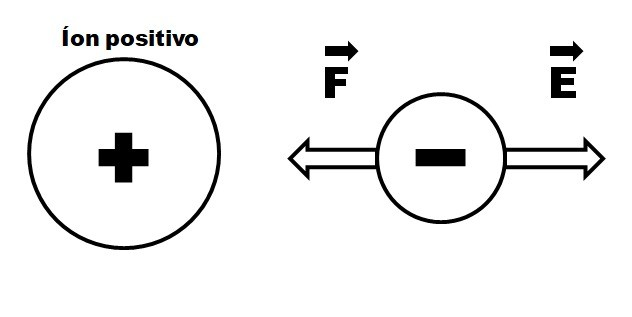
\includegraphics[width=0.5\textwidth]{forcas.jpeg}
    \fonte{Autoral}
\end{figure}

Analisando mais especificamente esse movimento, quando o elétron é deslocado e, em seguida, forçado a retornar a sua posição de origem, ele ganha uma certa energia cinética e, em virtude disso, acaba ultrapassando a posição de origem. Essa dinâmica é realizada consecutivas vezes, fazendo com que esse movimento se assemelhe a um movimento harmônico, ou seja, é aquele em que um corpo oscila em torno de uma posição de equilíbrio em razão de uma força restauradora (equação \ref{forca-restauradora}). Em primeiro momento, é de se admitir que o sistema é conservativo, logo o elétron terá comportamento análogo a um pêndulo simples, uma mola, ou uma onda sonora. Esta última, por sua vez, tem sua força restauradora originada pela pressão do gás, enquanto o objeto desse estudo (elétrons no plasma) tem por força restauradora as forças eletrônicas.

 Após o equacionamento da força restauradora e de seu desenvolvimento é possível encontrar a frequência natural do plasma e sua equação horária. Dentre desses resultados, pode-se inferir que a oscilação de elétrons ocorre tanto na ionosfera quanto nos metais em alta temperatura.

 Dentro desse contexto, a ionosfera sofre esse fenômeno devido aos raios ultravioleta do Sol, os quais arrancam elétrons livres das molécula de ar e produzem elétrons livres e íons positivos. Um dos efeitos que tal situação proporciona à ionosfera é que apenas ondas com frequências maiores que a do plasma conseguem atravessar a camada atmosférica, como por exemplos as ondas via satélite que são lançadas ao espaço. Outro ponto a se ressaltar é que as comunicações via rádio também são influenciadas por essa frequência natural do plasma contido na ionosfera, haja vista que, como as frequências de rádio são mais baixas, é possível que elas sejam refletidas pela ionosfera e, consequentemente, ampliem seu campo de atuação.

 Dando mais detalhamento a esse efeito reflexivo, é importante destacar que a propagação de ondas eletromagnéticas (como a luz) no plasma ionosférico, tem comportamento semelhante à ondas sônicas dentro de fluídos dentro de fluidos de diferentes densidades.

Nessa perspectiva, o índice de refração vai diminuindo com a altura, com camadas paralelas de densidade semelhantes, de acordo coma Lei de Snell, um incidente procedente da Terra, se curvará até atingir uma trajetória horizontal

\begin{figure}[htb]
    \caption{\label{refracao}Refrações sucessivas}
    \centering
    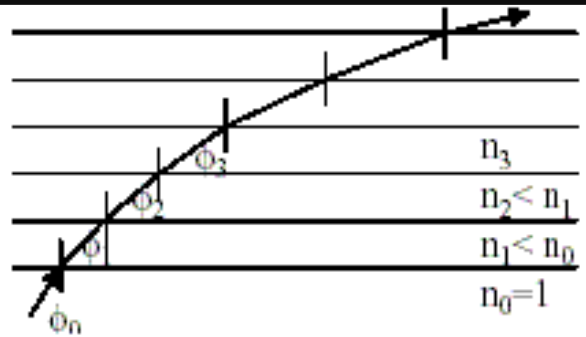
\includegraphics[width=0.5\textwidth]{refracao.png}
    \fonte{Wiki do IFSC\protect\footnotemark}
\end{figure}
\footnotetext{Disponível em \url{https://wiki.sj.ifsc.edu.br/wiki/images/3/36/4_0IFSC_Engenharia_ANT_2016_1.pdf}. Acesso em: 7 jun. 2021}

 Observe, na imagem acima, que a um raio oblíquo que passa por sucessivas refrações eventualmente atinge o ângulo limite. Nessa situação, ocorre o fenômeno de reflexão total.

 Em relação aos metais, existe uma densidade $n_o$ muito grande de partículas e, consequentemente, uma frequência natural muito elevada também. Ainda assim, há uma possibilidade de ``ver'' as oscilações dos elétrons. Conforme a mecânica quântica, uma frequência harmônica natural $\omega_p$, possui níveis de energia divididos por incrementos de energia $\hbar\omega_p$. Logo, se atirarmos alguns elétrons através de uma folha de alumínio, quando olharmos para os mesmos após a penetração e calcularmos os níveis de energia, será possível perceber que os elétrons terão perdido uma energia $\hbar\omega_p$ para as oscilações dos plasmas dos metais.

Além dos resultados obtidos, é possível ainda descrever um sistema no qual as oscilações harmônicas não são conservativos. Isso ocorre quando existe uma perda de energia gerada por atrito e por colisões entre os elétrons, que levam a dissipação de energia cinética em forma de calor. Nesse caso, podemos modelar a força resistiva como diretamente proporcional a velocidade, como visto na equação \ref{forca-amortecimento}. Utilizando esse modelo, fomos capazes de calcular a frequência natural desse sistema amortecido.

\section{Conclusão}

Após essa detalhada análise, concluímos que nosso método de modelagem matemática permitiu significativo avanço na representação analítica da situação física estudada. Essa representação, por sua vez, possibilitou melhor compreensão do comportamento do sistema físico, tanto do ponto de vista da dinâmica quanto da cinemática.

\nocite{feynman_leighton_sands_2009, halliday_resnick_walker_2008, mazur_et_al_2016}

\pagebreak
\onecolumn{
\postextual
\bibliography{references}
}

\end{document}
